\subsubsection{High Level View}
This section is dedicated to an overview of the architectural elements composing the CodeKata system and their most important interactions. 

The CKB system is built with a microservices architectural style. A microservices architectural style is a type of software architecture in which the application is developed as a collection of services, which are units of functionalities designed to cooperate with one another in order to achieve the goals for which the system is developed. In order to make this description as clear as possible, a high-level view of the system (with its microservices) is illustrated in the following image:
\begin{center}
\includegraphics[width=0.75\linewidth, page=2]{OverViewDiag}
\captionof{figure}{Overview of microservices and main interactions}
\end{center}


From a very high-level perspective, all the previously mentioned elements are also represented in this figure. The client is the first icon on the top, the \app system is represented as a set of hexagonal microservices, which also leverage external platforms, like GitHub and the Static Analysis Tool. Finally, at the very bottom, the data layer is shown with a database icon.

There are seven microservices in the \app system, each one offering some functionality, described as follows:

\begin{itemize}
	\item \textbf{Gateway Microservice}: this microservice is responsible for a couple of things. First off, the Gateway Microservice handles the authentication process of users through GitHub. From the figure, it's easy to spot the relationship between this microservice and GitHub external actor. Moreover, the Gateway handles all the incoming users' requests and dispatches them to the specific microservice that has to handle them. All users requests pass by the Gateway, as well as all responses of the system traverse the gateway to reach the users. In order to grant availability and performance, this microservice can be replicated multiple times on the server side of the application.
    \item \textbf{User Management Microservice}: this microservice is responsible for the management of users' data and profiles. Thus, the User Management Microservice controls the usernames of students and educators, as well as providing the user profile page every time a user accesses \app.
    
    \item \textbf{Tournament Microservice}: this microservice grants control over the tournaments and manages tournaments data in the shared database. It is responsible for the creation of a tournament from an educator, as it provides the user interface to do that. Besides, it maintains data on open tournaments, closed tournaments, tournaments rankings and so on. It is also responsible for providing the tournaments' home pages when requested.
    
    \item \textbf{Battle Microservice}: this is the microservice responsible for managing battles. It provides the interface to create a new battle to an educator requesting it, maintains all data related to battles and delivers the battle home page when requested. It is also responsible for handling teams of students, as well as keeping the rankings of battles updated.
    
    \item \textbf{GitHub Integration Microservice}: this microservice is in charge of handling all the API requests involving GitHub, apart from the login phase (delegated to the Gateway Microservice). More specifically, this microservice is very helpful when \app has to create a new GitHub repository for a battle, or when students code solutions must be downloaded from GitHub.
    
    \item \textbf{Score Computation Microservice}: the purpose of this microservice is to calculate the score to be assigned to a student code solution for a battle. In order to do so, this microservice uses the build automation scripts and test cases provided by the educator, calculates the time passed from the beginning of the battle and leverages the Static Analysis Tool as well.
    
    \item \textbf{Notification Microservice}: this microservice is concerned with all the notifications needed for tournaments and battles. The Notificaiton Microservice listens to events in the system (event-driven development) and produces notifications for students or educator.
\end{itemize}

As for the interactions between these microservices, they will be addressed in much greater detail in the following section of this document. 
For now, it is relevant to know that all communications going from the client to the \app platform and vice versa traverse the gateway. Also the several user interfaces which \app is composed of are provided by different microservices (concerned with the proper data related to the interface), but the transmission of these interface is always mediated by the gateway.

All microservices also expose a \textbf{RESTful API}, which is the access point to the data and functionalities they offer. Thus, microservices will interact with one another through this interfaces when necessary, and these details will be shown in the following views.

Furthermore, every microservice has access to the same \textbf{shared database}, thanks to the interfaces exposed by the DBMS system, but each component covers different types of manipulations and computations on this shared data space, which are dependent on the functionalities offered by the microservice in question.

The interactions that occur inside this system also rely on an \textbf{event-driven pattern}. This pattern allows components (microservices) to asynchronously produce events on an Event Bus (or Event Queue) and other components to consume (read) those events and take actions accordingly. Further details will be supplied in the following of the Design Document.